\documentclass[journal=jpcl,manuscript=letter,layout=traditional]{achemso}
\usepackage{amsmath,xcolor,graphicx,colortbl}
\usepackage{amssymb,soul,color}

\author{George Volonakis}
\affiliation[Department of Materials, University of Oxford]{Department of Materials, University of
Oxford, Parks Road OX1 3PH, Oxford, UK}

\author{Amir Abbas Haghighirad}
\affiliation[Department of Physics, University of Oxford]{Department of Physics, Clarendon Laboratory,
University of Oxford, Parks Road, Oxford OX1 3PU, United Kingdom}

\author{Rebecca L. Milot}
\affiliation[Department of Physics, University of Oxford]{Department of Physics, Clarendon Laboratory,
University of Oxford, Parks Road, Oxford OX1 3PU, United Kingdom}

\author{Weng H. Sio}
\affiliation[Department of Materials, University of Oxford]{Department of Materials, University of
Oxford, Parks Road OX1 3PH, Oxford, UK}

\author{Marina R. Filip}
\affiliation[Department of Materials, University of Oxford]{Department of Materials, University of
Oxford, Parks Road OX1 3PH, Oxford, UK}

\author{Bernard Wenger}
\affiliation[Department of Physics, University of Oxford]{Department of Physics, Clarendon Laboratory,
University of Oxford, Parks Road, Oxford OX1 3PU, United Kingdom}

\author{Michael B. Johnston}
\affiliation[Department of Physics, University of Oxford]{Department of Physics, Clarendon Laboratory,
University of Oxford, Parks Road, Oxford OX1 3PU, United Kingdom}

\author{Laura M. Herz}
\affiliation[Department of Physics, University of Oxford]{Department of Physics, Clarendon Laboratory,
University of Oxford, Parks Road, Oxford OX1 3PU, United Kingdom}

\author{Henry J. Snaith}
\affiliation[Department of Physics, University of Oxford]{Department of Physics, Clarendon Laboratory,
University of Oxford, Parks Road, Oxford OX1 3PU, United Kingdom}

\author{Feliciano Giustino}
\affiliation[Department of Materials, University of Oxford]{Department of Materials, University of
Oxford, Parks Road OX1 3PH, Oxford, UK}
\email{feliciano.giustino@materials.ox.ac.uk}\phone{(+44) 01865 272380 }

\title{Cs$_2$InAgCl$_6$: A New Lead-Free Halide Double Perovskite With Direct Band Gap}

\begin{document}
\newpage

\begin{abstract}

\noindent A$_2$BB$^\prime$X$_6$ halide double perovskites based on bismuth and silver have recently
been proposed as potential environmentally-friendly alternatives to lead-based hybrid halide perovskites.
In particular, Cs$_2$BiAgX$_6$ (X = Cl, Br) have been synthesized and found to exhibit band gaps in the
visible range. However, the band gaps of these compounds are indirect, which is not ideal for applications
in thin film photovoltaics. Here, we propose a new class of halide double perovskites, where the B$^{3+}$ and B$^{+}$
cations are In$^{3+}$ and Ag$^{+}$, respectively. Our first-principles calculations indicate that the hypothetical
compounds Cs$_2$InAgX$_6$ (X = Cl, Br, I) should exhibit direct band gaps between the visible (I) and
the ultraviolet (Cl). Based on
these predictions, we attempt to synthesize Cs$_2$InAgCl$_6$ and Cs$_2$InAgBr$_6$, and we succeed to
form the hitherto unknown double perovskite Cs$_2$InAgCl$_6$. X-ray diffraction yields
a double perovskite
structure with space group $Fm\overline{3}m$.
The measured band gap is 3.3~eV, and the compound is found to be photosensitive and turns reversibly from white to orange
under ultraviolet illumination.
We also perform an empirical analysis of the
stability of Cs$_2$InAgX$_6$ and their mixed halides based on Goldschmidt's rules, and we find that
it should also be possible to form Cs$_2$InAg(Cl$_{1-x}$Br$_{x}$)$_6$ for $x<1$. The synthesis of mixed
halides will open the way to the development of lead-free double perovskites with direct and tunable band gaps.


\end{abstract}


\newpage

During the last four years Pb-based halide perovskites have revolutionized the field of solution processable
solar cells, achieving record power conversion efficiencies above 22\%, and surpassing
polycrystalline and thin-film silicon photovoltaics (PV)~\cite{Xing2013,Stranks2013,
Seo2016,Eperon2016}. While
the efficiency of these materials improves steadily, there are two remaining challenges that need to
be addressed in order to use perovskite solar cells for electricity production, namely the compound
stability and the presence of lead~\cite{Green2014}. On the front of Pb replacement,
several lead-free perovskites and perovskite-derivatives have been proposed during the past two years
as potential substitutes for MAPbI$_3$ (MA = CH$_3$NH$_3$)~\cite{Giustino2016}, including vacancy-ordered double perovskites,
cation-ordered double perovskites (also known as elpasolites), and two-dimensional perovskites~\cite{Stoumpos2013,Noel2014,
Saparov2015,Kim2016,Xiao2016,Volonakis2016,Slavney2016,McClure2016,Filip2016b,Milot2016,Kaltzoglou2016}.
Among these compounds, Pb-free halide double perovskites based on Bi and Ag were recently proposed as stable and
environmentally-friendly alternatives to MAPbI$_3$~\cite{Volonakis2016,Slavney2016,McClure2016,Filip2016b}. While these
Bi/Ag double perovskites exhibit band gaps in the visible (from 1.9 to 2.2~eV~\cite{Filip2016b}), the gaps are {\it indirect},
which is not ideal for thin film PV applications. In fact indirect band gaps imply weak oscillator strengths for
optical absorption and for radiative recombination, therefore indirect semiconductors such as silicon need a much thicker absorber
layer, which can be problematic if charge carriers mobilities are low.
In order to circumvent this limitation, in this work we develop a new class of Pb-free halide double
perovskites, which exhibit {\it direct} band gaps. We first use available databases and
first-principles calculations to identify double perovskites with direct band gaps, and then we
synthesize and characterize the new In-based compound Cs$_2$InAgCl$_6$. X-ray diffraction (XRD) indicates
a double perovskite structure with space group $Fm\overline{3}m$ at room temperature, with a direct
band gap of 3.3~eV.

The starting point of our investigation is the recent work on Cs$_2$BiAgCl$_6$ by some of us~\cite{Volonakis2016}.
In that work we succeeded in synthesizing the new double perovskite
Cs$_2$BiAgCl$_6$ by following the well-known reaction route for making Cs$_2$BiNaCl$_6$~\cite{Morss1972},
and by replacing the NaCl precursor by AgCl. The successful replacement of Na by Ag can be attributed
to the close match between the ionic radii of Na$^{+}$ (1.02~\AA) and of Ag$^{+}$ (1.15~\AA).
Motivated by this observation, here we set to discover new halide double perovskites containing
Ag. To this aim we search for known halide elpasolites containing Na$^{+}$ as the B$^{+}$ cation.
We consider data from the Materials Project~(www.materialsproject.org), the International Crystal
Structure Database (ICSD), and literature reviews~\cite{Morss1970,
Morss1972,Meyer1978,Meyer1980}. We find 42
elpasolites with composition Cs$_2$B$^{3+}$NaX$_6$, X = Cl, Br, I. In 30 of these compounds
the B$^{3+}$ cation is a lanthanide or actinide; in 7 compounds we find transition metals
with small ionic radii ($<$0.9~\AA), namely Sc, Ti, Y, and Fe; and 5 compounds
contain Bi, Sb, Tl, or In. Lanthanides, actinides and transition metals pose a challenge to computational
predictions based on DFT, therefore we leave them aside for future
work. Bi and Sb double perovskites were extensively discussed recently~\cite{Volonakis2016}.
The incorporation of Tl in halide double perovskites was also proposed~\cite{Giorgi2015},
however this element is highly toxic and hence unsuitable for optoelectronic applications.
Indium, on the other hand, is a common element in the optoelectronic industry, for example
it is used to make transparent conductors in the form of tin doped indium oxide (ITO).
Two In/Na-based halide double perovskites have been reported so far, Cs$_2$InNaCl$_6$~\cite{Morss1970,
Meyer1978} and Cs$_2$InNaBr$_6$~\cite{Meyer1978}. Following this observation, we proceed to
assess the structural, electronic, and optical properties of the hypothetical compounds
Cs$_2$InAgX$_6$ with X = Cl, Br, I using DFT calculations.



As a structural template for our calculations we use the face-centered cubic $Fm\bar{3}m$
elpasolite unit cell, which contains one B$^{+}$X$_6$ and one B$^{3+}$X$_6$
octahedra~\cite{Volonakis2016,McClure2016}. The resulting atomistic model consists of
InX$_6$ and AgX$_6$ octahedra which alternate along the [100], [010], and [001] directions,
as shown in Figure~\ref{fig:1}a. This rock-salt ordering of the B-site cations is also found
in many oxide double perovskites. After optimizing the structure within
the local density approximation (LDA) to DFT (see Methods), we obtain the lattice constants
$a=10.20$~\AA, $10.74$~\AA, and $11.52$~\AA\ for X = Cl, Br, and I, respectively.
The calculated lattice constants are slightly smaller than what we found for the corresponding
Bi-based double perovskites (10.50-11.76~\AA)~\cite{Volonakis2016}. This can
be attributed to the smaller size of In$^{3+}$ as compared to Bi$^{3+}$. Despite the presence
of two different B-site cations, within DFT/LDA the BX$_6$ octahedra are of similar
size; for example in the case of Cs$_2$InAgCl$_6$ the In-Cl and Ag-Cl bond lengths are 2.50~\AA\
and 2.59~\AA, respectively. Employing higher level non-local functionals for
the structural optimization yields a slightly larger lattice constant, 10.62~\AA\ for Cs$_2$InAgCl$_6$,
and bond lengths of 2.54~\AA\ and 2.77~\AA\ for In-Cl and Ag-Cl, respectively.
All parameters related to structural optimization with different functionals are included
in Table S1 of the Supporting Information.


A complete study of the stability of these hypothetical compounds would require the calculation
of the phonon dispersion relations (dynamical stability) and of the quaternary convex hulls
(thermodynamic stability)~\cite{Hautier2012}. Since these
calculations are demanding, we perform a preliminary assessment of compound stability using
Goldschmidt's empirical criteria. According to these criteria, one can
assign a perovskite with formula ABX$_3$ two parameters called the tolerance factor and the octahedral
factor. The tolerance factor is defined as $t = (R_{\rm A}+R_{\rm X})/\sqrt{2}
(R_{\rm B}+R_{\rm X})$, with $R_{\rm A}$, $R_{\rm B}$, and $R_{\rm X}$ the ionic radii of the
elements in a ABX$_3$ perovskite; stable structures usually correspond to $0.75<t<1.0$~\cite{li}.
The octahedral factor is defined as $\mu = R_{\rm B}/R_{\rm X}$,
and stable structures tend to have $\mu > 0.41$.
In order to evaluate these parameters we employ the Shannon ionic radii.
Since we have double perovskites, and therefore different radii for the B$^{+}$  and B$^{3+}$
sites, as a first attempt we consider for $R_{\rm B}$ the average between the radii of In$^{3+}$ and Ag$^{+}$.
For Cs$_2$InAgX$_6$ with X = Cl$^{-}$, Br$^{-}$, I$^{-}$ we obtain $(\mu,t) = (0.54,0.94)$, (0.50,0.93), and
(0.44,0.91), respectively. All these parameters fall within the range of stability of
standard halide perovskites~\cite{li}, therefore they are not very informative. A more stringent
test can be obtained by considering the limiting cases where the structures were composed
entirely of InX$_6$ octahedra or of AgX$_6$ octahedra. In this scenario we find that
the tolerance factor is within the stability region for all compounds ($0.86<t<1.0$), but the octahedral
factor $\mu$ is outside of this region for X = Br and I. The evolution of the octahedral
factor as one moves from Cs$_2$InAgCl$_6$ to Cs$_2$InAgI$_6$ is shown in Figure~\ref{fig:1}b.
It is apparent that the onset of the instability relates to the InX$_6$ octahedra, and in
particular to the fact that the ionic radius of In$^{3+}$ is too small ($R_{{\rm In}^{3+}}=0.8$~\AA)
to coordinate 6~I$^{-}$ anions ($R_{{\rm I}^{-}}=2.2$~\AA).
This analysis, albeit very crude, suggests that the only possible In/Ag halide double
perovskites that may be amenable to synthesis are those with Cl, Cl/Br mixes, and possibly Br.



Guided by these results, we investigate the electronic structure of Cs$_2$InAgCl$_6$.
In order to overcome the well-known limitations of DFT/LDA for the description of band gaps,
we employ the HSE and the PBE0 hybrid functionals (see Methods). We also checked that,
unlike in MAPbI$_3$~\cite{Even2013}, spin-orbit effects are not important for In/Ag double perovskites,
see Figure~S1 of the Supporting Information. The band structure of Cs$_2$InAgCl$_6$ is shown
in Figure~\ref{fig:2}a. The most striking finding is that the band gap is {\it direct},
with both valence and conduction band extrema at the center of the Brillouin zone ($\Gamma$ point).
The band gap is rather sensitive to the functional
employed for the structural optimization (see Table~S1), and ranges from 2.1~eV (LDA structure,
HSE gap) to 3.3~eV (HSE structure, PBE0 gap). Given this uncertainty, we choose to report
$2.7\pm0.6$~eV as the nominal band gap from the calculations. In Table~1 we
show the previously calculated~\cite{Volonakis2016,Filip2016b} and measured
\cite{Volonakis2016,Filip2016b,Slavney2016,McClure2016} band gaps for the case of Cs$_2$BiAgX$_6$
(X = Cl, Br). The measured band gaps are within the HSE-PBE0 range, hence we expect a similar trend
for Cs$_2$InAgCl$_6$.

In Figure~\ref{fig:2}b we show the square modulus of the electronic wavefunctions at the band
edges. The bottom of the conduction band is mainly comprised of Cl-$3p$ and In-$5s$/Ag-$5s$ states,
while the top of the valence band is derived from Cl-$3p$ and In-$4d$/Ag-$4d$ states.
A detailed projected density of states and a qualitative molecular orbital diagram of
Cs$_2$InAgCl$_6$ are shown in Figure~S2 of the Supporting Information.
The valence band top of Cs$_2$InAgCl$_6$ has no occupied In-$s$ orbitals. This  is closely
linked with the direct character of the band gap of this
compound. In fact, in the related Bi/Ag elpasolite Cs$_2$BiAgCl$_6$~\cite{Volonakis2016,Filip2016b},
the Bi $s$ states at the top of the valence band interact with the directional Ag $d$ states
along the [100] direction; this interaction pushes the valence band top to the $X$ point
and leads to an indirect band gap in Cs$_2$BiAgCl$_6$. To confirm this point we artificially removed the
Bi $s$ states from the top of the valence band of  Cs$_2$BiAgCl$_6$, using a fictitious
Hubbard $U$ correction of 10~eV. The resulting band structure, shown
in Supporting Figure~S3, exhibits a direct gap at $\Gamma$, as in the case of the
present compound Cs$_2$InAgCl$_6$.

The electron effective mass calculated for Cs$_2$InAgCl$_6$ is $m^*_{\rm e}=0.29\,m_{\rm e}$
($m_{\rm e}$ is the free electron mass); the hole effective mass is $m^*_{\rm h}=0.28\,m_{\rm e}$.
In the calculation of the hole effective mass we have not considered the non-dispersive
band which can be seen in Figure~\ref{fig:2}a between $\Gamma$ and X.
This flat band originates from the hybridization of Cl-$3p_{x,y}$ states and
$4d_{x^2-y^2}$ states of In and Ag, which leads to a two-dimensional wavefunction confined
within the equatorial (001) plane (wavefunction labelled as `iii' in Figure~2b).
This flat band will likely prevent carrier
transport along the six equivalent $X$ wavevectors, and possibly favor the formation
of deep defects.



Since we expect Cs$_2$InAgCl$_6$ to be stable, and to exhibit a direct band gap as well
as small and balanced effective masses, we proceed to attempt the synthesis of this compound.
We prepare samples of Cs$_2$BiAgCl$_6$ by precipitation from an acidic solution of hydrochloric
acid. A mixture of a 1~mmol InCl$_3$ (Sigma Aldrich, 99.99\%) and AgCl (Sigma Aldrich, 99\%) is
first dissolved in 5~mL 10~M HCl. Then 2~mmol of CsCl (Sigma Aldrich, 99.9\%) are added and
the solution is heated to 115~$^\circ$C. A white precipitate forms immediately after adding CsCl.
We leave the hot solution for 30~min under gentle stirring, to ensure a complete reaction
before filtering. We wash the resulting solid with ethanol and dry in a furnace overnight
at 100~$^\circ$C. The as-formed powder appears stable under ambient conditions. In Figure~\ref{fig:3}a
we show the measured X-ray diffraction (XRD) pattern of this powder. The refined lattice parameter
is 10.47~\AA, only 2.6\% larger than in our DFT/LDA calculation. This is in line with the typical
underestimation of lattice parameters by DFT/LDA in the range of 1-2\%.
The refined structural parameters are provided in Table~S2 of the Supporting Information.
In Figure~\ref{fig:3}a we include the powder diffraction pattern calculated from our optimized
DFT/LDA structure. We can see that all the peaks in the calculation and in the XRD measurement
match very closely; there is a small offset between the two patterns, which is related to the
difference in the lattice parameters. To confirm this point, we re-optimize the theoretical model using
the experimental lattice constant; in this case we find no discernible difference between the
two patterns, as shown in Figure~S4a of the Supporting Information. This comparison indicates that
the synthesized compound is a double perovskite or elpasolite, within a $Fm\bar{3}m$
space group. We also measured the XRD pattern after exposing the samples to ambient conditions for
more than three months, as shown in Figure~S5 of the Supporting Information. The compound
appears to be very stable with no structural decomposition observed. While we can
successfully synthesize Cs$_2$InAgCl$_6$, our preliminary attempts at making
the related bromide compound, Cs$_2$InAgBr$_6$, have been unsuccessful thus far. In fact, by
following a similar route as above, with CsBr instead of CsCl, we obtain a pale yellow powder that
does not match the elpasolite $Fm\overline{3}m$ crystal structure.

In order to investigate whether the In and Ag cations are fully ordered,
we have calculated the XRD pattern in three different
scenarios: (1) using an ordered structure optimized within DFT/LDA, (2) using an ordered structure
optimized with DFT/HSE, (3) using the measured lattice parameter and a perovskite structure with
0.5 In and 0.5 Ag occupations on the Wyckoff sites. The scenarios (1) and (2) are meant to
describe a fully-ordered Cs$_2$InAgCl$_6$ crystal using DFT functionals which
yield rather different In-Cl and Ag-Cl bond lengths (as shown in Table~S1).
These calculated XRD patterns are compared to experiment in Figure~S6 of the Supporting Information.
The main peaks associated with ordering effects are indicated by the green arrows in this figure.
We find that the main peaks associated with ordering effects (indicated by the green arrows)
are extremely weak even in the theoretical fully-ordered structures.
Furthermore, we see that in the HSE structure these peaks are slightly more visible than in the LDA
structure. This effect is due to the more pronounced difference in bond lengths between In-Cl and Ag-Cl
in the HSE structure (as seen in Table~S1). In the fully-disordered model the intensity of the
ordering peaks is vanishing.
The difference between the XRD patterns calculated for the ordered structures (Figure~S6b and~S6c)
and the disordered structure (Figure~S6d) are much smaller than our experimental resolution (Figure~S6a).
Therefore, in the case of
Cs$_2$InAgCl$_6$, XRD is not sufficient to probe the nature of cation order/disorder.
Given this uncertainty on the structure, we explored the
effects of disorder on the electronic structure. To this aim we considered a virtual crystal
approximation with the In and Ag sites replaced by the pseudo-atom 0.5 In + 0.5 Ag.
As shown in Figure~S7, the DFT/HSE band structure of this disordered model
is very close to that of the ordered model, with the same direct band gap at $\Gamma$.
This demonstrates that our electronic structure analysis should be mostly insensitive to cation
ordering.

In order to characterize the optical properties of Cs$_2$InAgCl$_6$, we measured the diffuse
reflectance and applied the Kubelka-Munk theory (see Methods) to estimate the absorbance, and
the time-resolved photoluminescence (PL) spectra. The Kubelka-Munk function $F(R)$
is shown in Figure~\ref{fig:3}b. We can clearly recognize the onset
of absorption near 380~nm (3.3~eV) and further identify a second absorption feature
at 585~nm (2.1~eV). The full reflectance spectra is shown in Figure~S8 of the Supporting Information.
In Figure~\ref{fig:3}c we see a well-defined PL peak centered around 608~nm (2.04~eV), with a
FWHM of 120~nm (0.37~eV).This peak appears to redshift on a timescale of 100~ns, suggesting that
subgap states are being filled on this timescale.

A compound with the absorption onset and PL peak close to 2.1~eV should be colored orange
and not white as the Cs$_2$InAgCl$_6$ powder. However, we have observed that under photo-excitation
the compound turns orange as shown in the insets of Figure~\ref{fig:3}b.
This coloration might relate to local
photo-induced electronic or structural changes. For example, the precursor compound AgCl is a known
photosensitive material, where the oxidation state of Ag changes upon illumination.
This photochromic behavior may be connected with the strong sensitivity of the electronic
structure of Cs$_2$InAgCl$_6$ to small changes in the Ag-Cl and In-Cl bond lengths,
as shown in Table~S1 of the Supporting Information.
The process observed here
is fully reversible and upon return to ambient light the sample becomes immediately white.
The orange coloration
is consistent with the optical absorption around 2.1~eV and the emission spectra shown
in Figure~3b and c. Based on these observations we propose that the measured absorption and
emission around 2.1~eV might relate to (possibly photo-induced) defect states, and the
actual band gap of the compound is at 3.3~eV.



In Figure~\ref{fig:3}d we see
that the time-resolved PL intensity of Cs$_2$InAgCl$_6$ exhibits two timescales, a fast
relaxation with a lifetime of 1~ns, followed by a very slow decay with a long lifetime of
6~$\mu$s. This observation is consistent with time-resolved PL measurements on the
related Cs$_2$BiAgX$_6$ (X = Cl, Br) double perovskites, which also exhibit two decay
components with very different lifetimes~\cite{Slavney2016}.
For completeness in Figure~S4b of the Supporting Information we show that the PL lifetime
is insensitive to the intensity of the pump laser. Taken together, the PL redshift with time,
and the fast initial PL decay component suggest that a tail of
subgap defect states or energetic disorder is present.



We now employ DFT to compare the {\it ideal} optical absorption spectrum of Cs$_2$InAgCl$_6$ and
Cs$_2$InAgBr$_6$ with the spectra calculated for the standard semiconductors Si and GaAs,~\cite{Marios2016}
and for MAPbI$_3$ (unpublished results). In Figure~\ref{fig:4}a we see that, while
Cs$_2$InAgCl$_6$ is a direct-gap semiconductor, the absorption coefficient of the perfect crystal is considerably
smaller than those of Si, GaAs, and MAPbI$_3$ throughout the visible spectrum. On the other hand,
if we could synthesize an ideal crystal of the bromine compound, Cs$_2$InAgBr$_6$, we should obtain
an absorption coefficient which is comparable or even higher than in silicon.

In view of developing more efficient absorbers based on the In/Ag combination, we theoretically
investigate the optical properties of mixed halide compounds. To this aim we consider the hypothetical solid solutions
Cs$_2$InAg(Cl$_{1-x}$Br$_{x}$)$_6$, Cs$_2$InAg(Br$_{1-x}$I$_{x}$)$_6$ and Cs$_2$InAg(Cl$_{1-x}$I$_{x}$)$_6$
with $x= 0.25$, 0.50, and 0.75. To model mixed-halide double perovskites without inducing
artificial ordering effects, we employ the virtual-crystal approximation (see Methods).
Figure~\ref{fig:4}b shows a ternary map of the band gap calculated for these mixes, as obtained
by interpolating linearly from the above combinations. We report band gaps calculated using
DFT/HSE  and DFT/PBE0  for Cs$_2$InAgCl$_6$. The band gaps of the mixed halide double perovskites
are  tunable within the visible spectrum. These results indicate
that the the In/Ag halide double perovskites may be promising for applications in tandem solar cell
architectures~\cite{Eperon2016}.

In summary, by combining first-principles calculations and experiments we discovered a novel
direct band gap halide double perovskite, Cs$_2$InAgCl$_6$. This new compound crystallizes in
a double perovskite structure with space group $Fm\bar{3}m$, has a direct band gap at $\Gamma$
of 3.3~eV. In addition, this new compound exhibits PL at around 2.1~eV and
shows an interesting photochromic behavior whereby the color changes reversibly to orange under
UV illumination. Our analysis indicates
that by developing mixed halides Cs$_2$InAgX$_6$ with X = Cl, Br, and I, it should be possible
to obtain good optical absorbers with tunable and direct band gaps.
The existence of the related compound Cs$_2$InNaBr$_6$ (with Na in place of Ag) strongly suggests
that it should be viable to synthesize also Cs$_2$InAgBr$_6$. Overall, we expect that the exploration
of mixed-halide double perovskites starting from Cs$_2$InAgCl$_6$ will offer new opportunities for
developing environmentally friendly perovskite photovoltaics and optoelectronics.

\vspace{0.5 cm}
\noindent{\it Computational Methods:}
Structural optimization was carried out within DFT using the Quantum ESPRESSO suite~\cite{QE-2009}.
Ultrasoft pseudopotentials~\cite{Rappe,Vanderbilt} were used to describe the electron-ion interaction,
and exchange-correlation effects were taken into account within the LDA~\cite{Ceperley,Perdew}.
The planewaves kinetic energy cutoffs were set to 35~Ry and 280~Ry for the electronic wavefunctions
and the charge density, respectively. The Brillouin zone was sampled using a 15$\times$15$\times$15
unshifted grid. The thresholds for the convergence of forces and total energy were set to 10$^{-3}$~Ry
and 10$^{-4}$~Ry, respectively. In order to overcome the DFT band gap problem we employed hybrid functional
calculations as implemented in the VASP code~\cite{vasp}. We used the PBE0 functional~\cite{pbe0}
and the HSE06 functional~\cite{HSE06}. In the latter case we set the screening parameter to 0.2~\AA$^{-1}$
and we used a mixing of 25\% of Fock exchange with 75\% of PBE exchange. In the hybrid calculations
we used the projector augmented wave method~\cite{paw}, with a 400~eV kinetic energy cutoff.
In the hybrid calculations the Brillouin zone was sampled using a 6$\times$6$\times$6 unshifted grid
for Cl or Br. For the I-based compound, Cs$_2$InAgI$_6$, DFT/LDA yields a spurious band crossing
and the resulting band structure is metallic. In this case, in order to perform hybrid calculations
we sampled the Brillouin zone using a 2$\times$2$\times$2 shifted grid.
We verified the correctness of the results by repeating the
same procedure for Cs$_2$InAgCl$_6$. For the calculations of the optical absorption coefficients
we used the YAMBO code~\cite{Yambo} within the random-phase approximation. In this case we used
norm-conserving pseudopotentials~\cite{TM} (with kinetic energy cutoff of 120~Ry), the PBE~\cite{pbe}
generalized gradient approximation, and a dense Brillouin zone grid with 40$\times$40$\times$40 points.
In order to correct for the band gap underestimation in DFT/PBE we used scissor corrections as
obtained from our HSE/PBE0 calculations. The optical $f$-sum rule was maintained by scaling the
oscillator strengths~\cite{Zacharias2015}.
The calculations based on the virtual-crystal approximation were performed by using
the procedure of Bellaiche and Vanderbilt~\cite{VCA}.

\noindent{\it Experimental Methods:}
Powder XRD was performed using a Panalytical X'pert diffractometer (Cu-K$\alpha_1$ radiation;
$\lambda = 154.05$~pm) at room temperature. Structural parameters were obtained by Rietveld refinement
using the General Structural Analysis Software~\cite{Larson2000,Toby2001}.
A Varian Cary 300 UV-Vis spectrophotometer with an integrating sphere was used to acquire diffuse
reflectance. To estimate the visible light absorption spectrum, we apply the Kubelka-Munk theory
to convert the diffuse reflectance in the $F(R)$ function, $F(R) = (1-R)^2/2R = K/S$, where
$R$ is the absolute reflectance of the sample, $K$ is the molar absorption coefficient, and
$S$ is the scattering coefficient.Time-resolved PL spectra were recorded following laser excitation at
405~nm, at a repetition rate of 10~MHz (Picoquant, LDH-D-C-405M). The PL signal was collected and directed
toward a grating monochrometer (Princeton Instruments, SP-2558), and detected with a photon-counting
detector (PDM series from MPD).

\begin{acknowledgement}
The authors are grateful to Marios Zacharias for sharing
the calculated absorption coefficients of Si, GaAs and MAPbI$_3$.
The research leading to these results has received funding from the Graphene Flagship (Horizon 2020
grant no. 696656 - GrapheneCore1), the Leverhulme Trust (Grant RL-2012-001), the UK Engineering and
Physical Sciences Research Council (Grant No. EP/J009857/1, EP/M020517/1 and EP/L024667/1). The authors
acknowledge the use of the University of Oxford Advanced Research Computing (ARC) facility
(http://dx.doi.org/10.5281/zenodo.22558) and the ARCHER UK National Supercomputing Service under
the `AMSEC' Leadership project and PRACE for awarding us access to the Dutch national supercomputer
'Cartesius'.
\end{acknowledgement}

\vspace{0.6cm}

{\bf Supporting Information: } Figures of the molecular orbital diagram and projected density of states for
Cs$_2$InAgCl$_6$, XRD-data of a sample exposed to ambient conditions for three months, measured reflectance
and Kubelka-Munk function and additional figures relevant to the in-text discussions about spin-orbit coupling
and the octahedra ordering effects. Tables showing the DFT structural parameters and calculated band gaps, and
Rietveld refinement of Cs$_2$InAgCl$_6$. This material is available free of charge via the Internet
http://pubs.acs.org.

\vspace{0.6cm}

\bibliography{bibliography}

\newpage

\begin{figure}[ht!]
\begin{center}
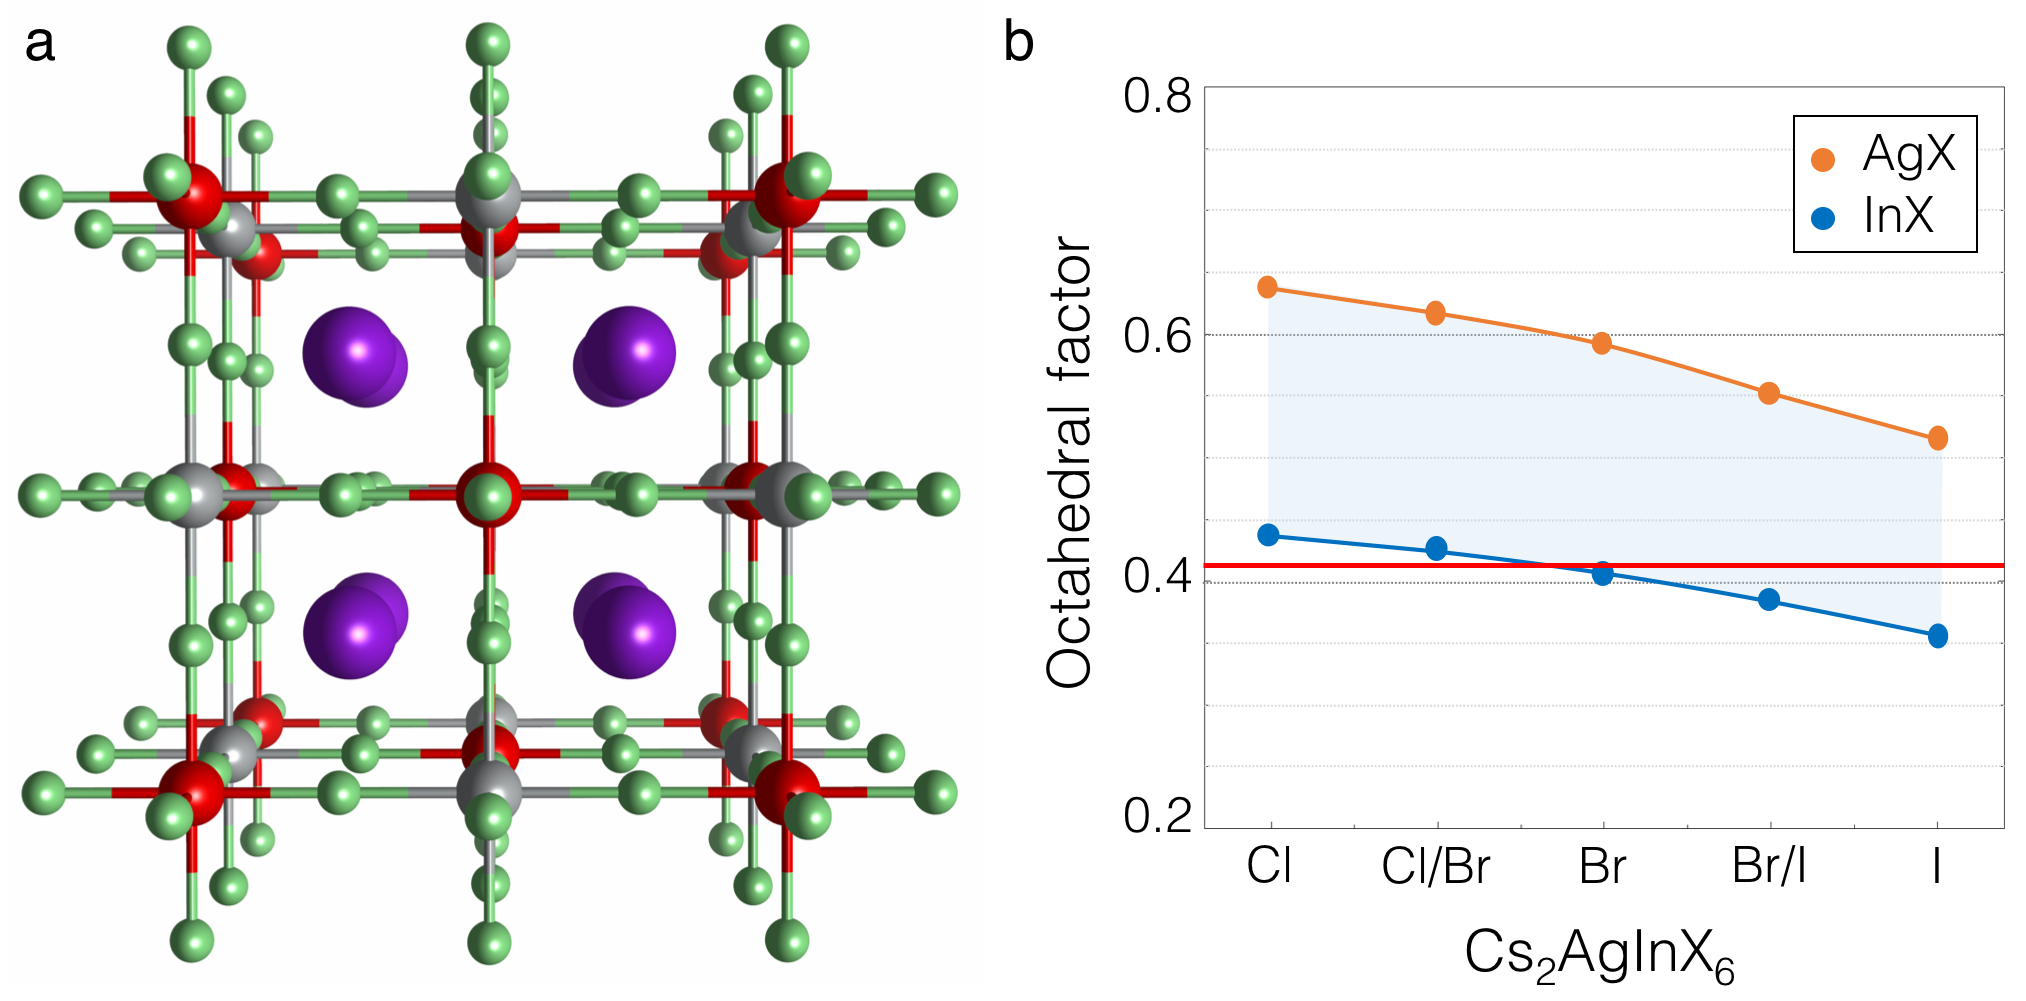
\includegraphics[width=0.75\textwidth]{figure1.png}
\end{center}
\caption{\label{fig:1}
   Atomistic model and octahedral factors of the In-based halide double perovskites Cs$_2$InAgX$_6$
   (X = Cl, Br, I): (a) Ball-and-stick model of Cs$_2$InAgCl$_6$, with In atoms in red and Ag atoms
   in gray. The green spheres indicate Cl, and the purple spheres in the center of each cavity are Cs atoms.
   The primitive unit cell contains one InCl$_6$ and one AgCl$_6$ octahedra in a face-centered cubic
   structure, with space group $Fm\overline{3}m$; here we show the conventional cubic cell.
   (b) Octahedral factor $\mu = R_{\rm B}/R_{\rm X}$ corresponding to AgX$_6$ octahedra (orange dots),
   and to InX$_6$ octahedra (blue dots), for solid solutions of Cl, Br, and I. The perovskite structure
   is expected to be unstable for values of the octahedral factor below $\mu = \sqrt{2}-1 = 0.41$,
   as indicated by the red horizontal line~\cite{li}.
   }
\end{figure}

\newpage

\begin{figure}[ht!]
\begin{center}
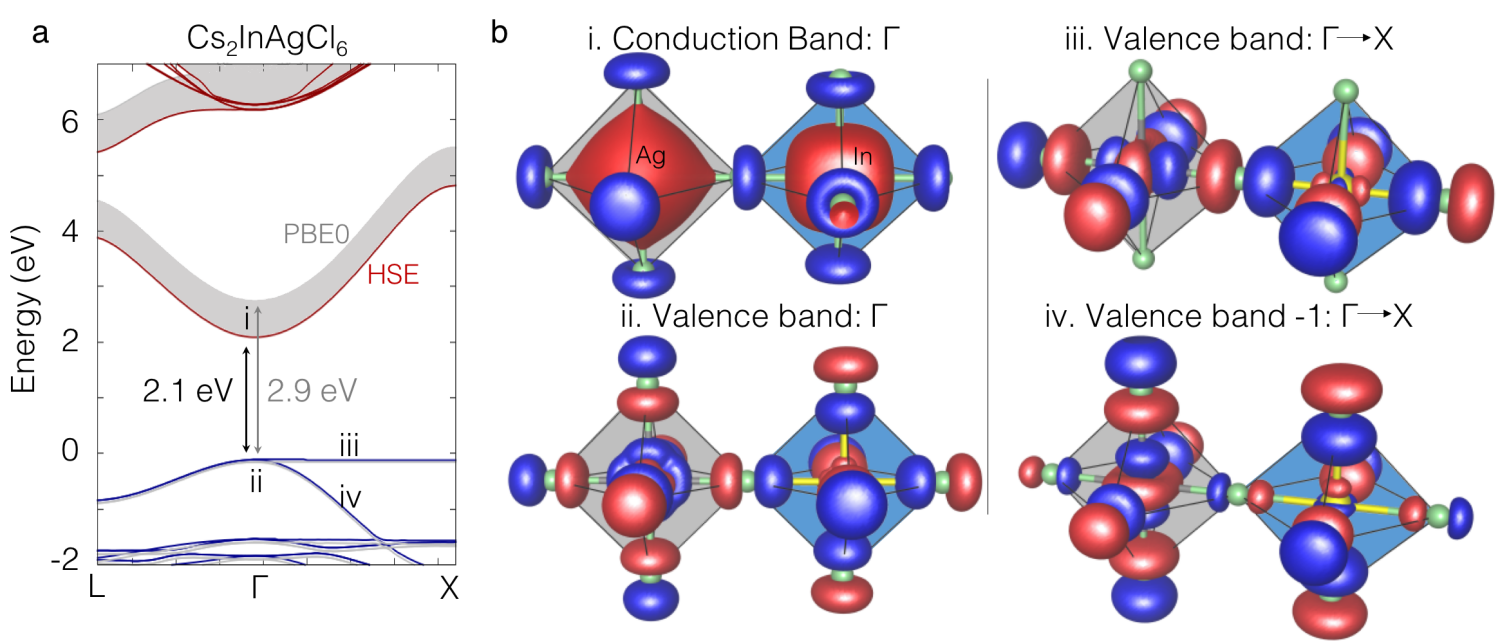
\includegraphics[width=0.9\textwidth]{figure2.png}
\end{center}
\caption{\label{fig:2}
  Electron band structure and square modulus of the wavefunctions for Cs$_2$InAgCl$_6$: (a) Band
  structures and band gaps of Cs$_2$InAgCl$_6$, as calculated by using the HSE hybrid functional
  (blue and red lines) or the PBE0 functional (shaded area). The zero of the energy scale is set to the top of
  the valence band. (b) Isosurface plots of the square modulus of the Kohn-Sham  wavefunctions corresponding to (i)
  the bottom of the conduction band at $\Gamma$; (ii) the sum of the two degenerate states at the valence band top
  at $\Gamma$; (iii) the highest occupied state along the $\Gamma$X line, for a wavevector ${\bf k}\rightarrow\Gamma$
  (0.2~$\Gamma$X); the second-highest occupied state along $\Gamma$X, for ${\bf k}\rightarrow\Gamma$ (0.2~$\Gamma$X).
  }
\end{figure}
\newpage

\begin{figure}[ht!]
\begin{center}
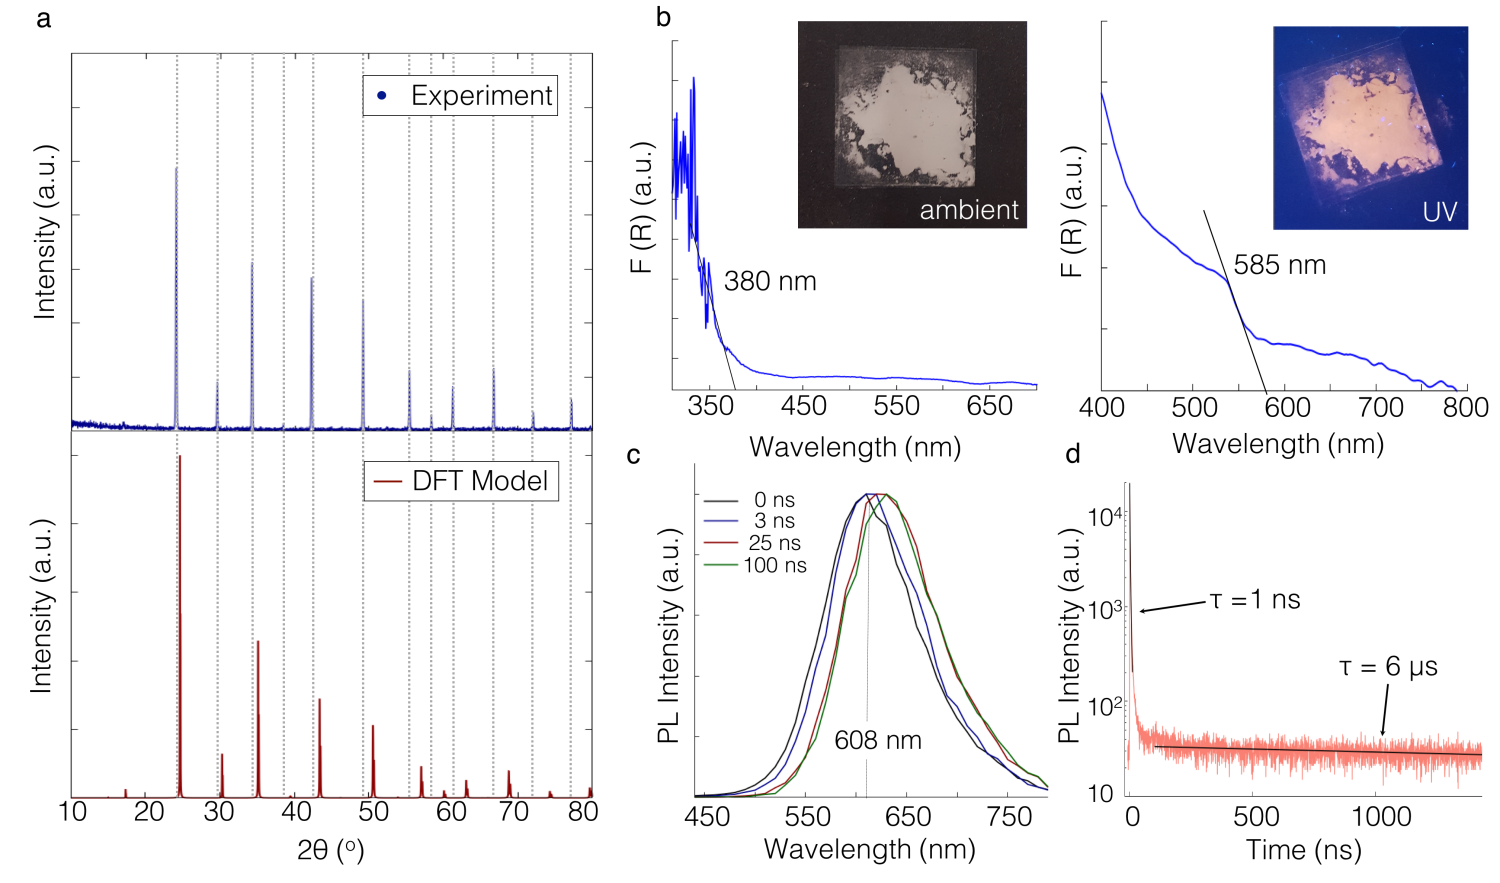
\includegraphics[width=1.0\textwidth]{figure3.png}
\end{center}
\caption{\label{fig:3}
  Structural and optical characterization of Cs$_2$InAgCl$_6$:
  (a) Measured powder XRD pattern for the as-synthesized Cs$_2$InAgCl$_6$ (top),
  and the XRD pattern calculated from the atomistic model optimized using DFT/LDA (bottom).
  (b) Measured UV-Vis absorbance showing the band gap of Cs$_2$InAgCl$_6$ at 380~nm and
  the defect-related features at 585~nm as discussed in-text. The straight lines are a guide to the eye.
  The insets shows Cs$_2$InAgCl$_6$ under ambient light and under
  UV illumination. (c) Normalized PL spectrum recorded as a function of time following
  excitation at 405~nm. The vertical line
  indicates the centre wavelength of the PL at zero time, defined by the arrival time of the excitation
  pulse on the sample. (d)
  Time-resolved PL intensity recorded for a powder sample of Cs$_2$InAgCl$_6$. The fast and slow components of the
  PL decay are indicated on the plot. The fast (slow) component was fit with a stretched exponential (monoexponential)
  function, and $\tau$ represents the average lifetime.
  }
\end{figure}
\newpage

\begin{figure}[ht!]
\begin{center}
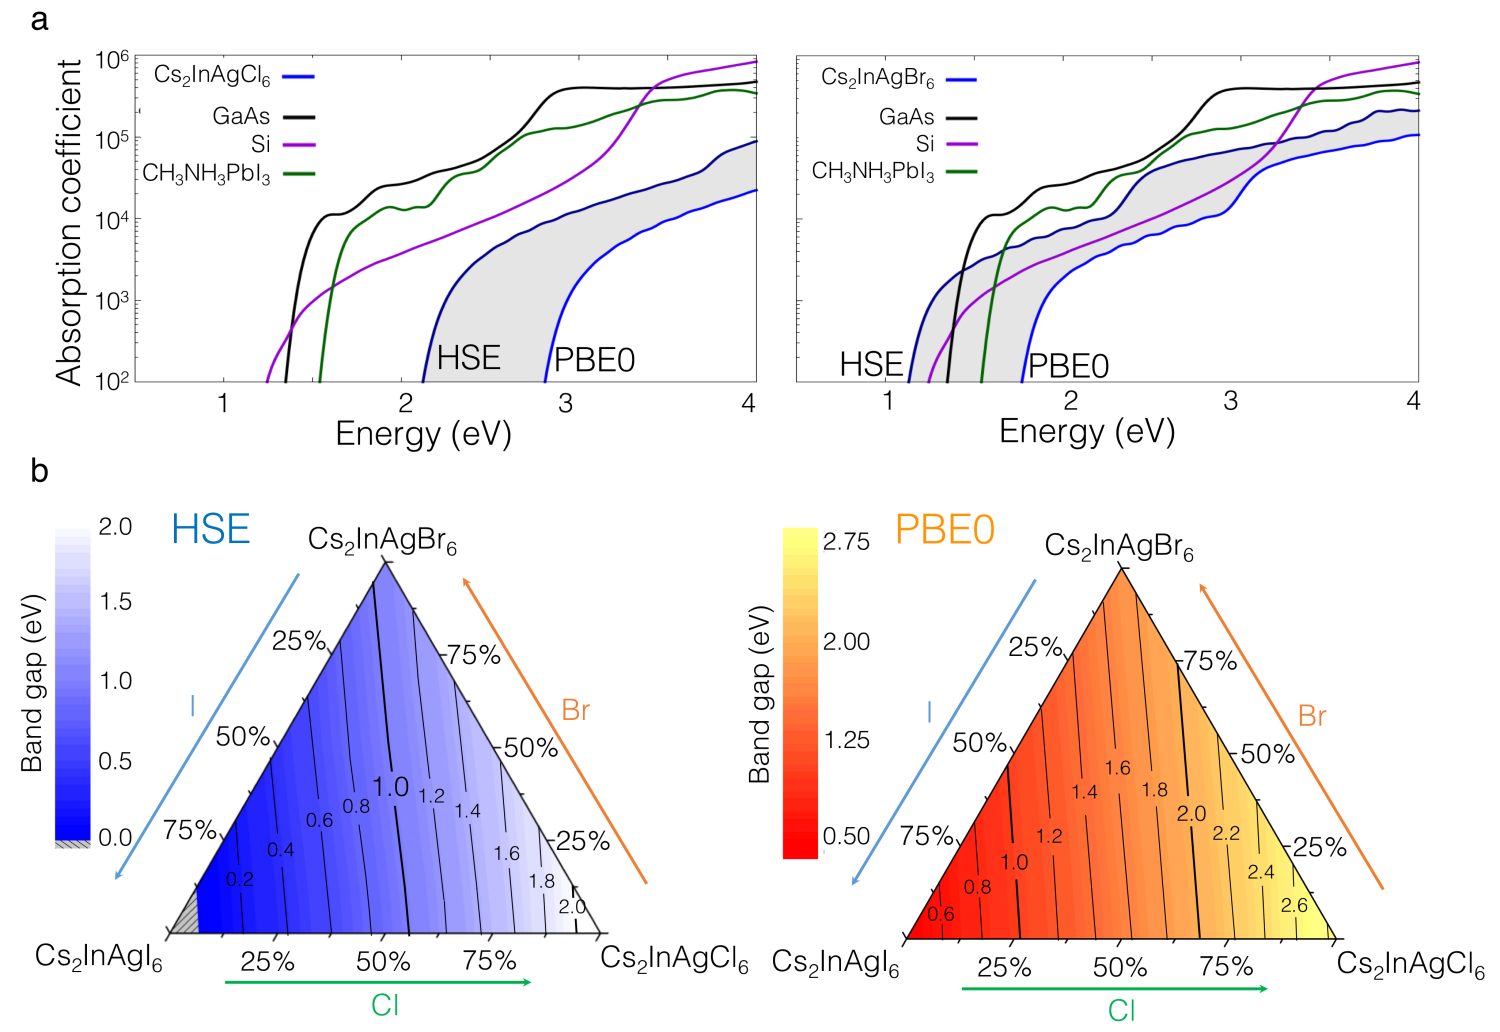
\includegraphics[width=0.85\textwidth]{figure4.png}
\end{center}
\caption{\label{fig:4}
  Theoretical optical absorption coefficient and band gap of mixed halides: (a) Calculated
  absorption coefficient of the compound synthesized in this work, Cs$_2$InAgCl$_6$ (left, blue lines),
  and of the hypothetical compound Cs$_2$InAgBr$_6$ (right, blue lines). For comparison we show the
  theoretical absorption coefficients of silicon (purple), gallium arsenide (black),
  as calculated in Ref.~\citenum{Marios2016}, and MAPbI$_3$
  (green) (unpublished results). (b)  Calculated
  band gaps of hypothetical mixed-halide double perovskites Cs$_2$InAg(Cl$_{1-x-y}$Br$_x$I$_y$)$_6$
  within the HSE (left) and PBE0 (right) hybrid functional. The corners of the triangle correspond
  to Cs$_2$InAgX$_6$ with X = Cl, Br, I.
  }
\end{figure}

\newpage

\begin{table}[t!]
\begin{center}
\caption{Comparison between calculated and measured band gaps of halide double perovskites:
  The first column reports our present results for Cs$_2$InAgCl$_6$ (HSE and PBE0 calculations;
  the range corresponds to different structural relaxations as detailed in Table~S1),
  the second and third columns report PBE0 calculations and measurements on Cs$_2$BiAgCl$_6$ and
  Cs$_2$BiAgBr$_6$ from Refs.~\citenum{Volonakis2016},~\citenum{Slavney2016}, ~\citenum{McClure2016}
  and~\citenum{Filip2016b}. The HSE calculations are from this work.}
  \setlength{\tabcolsep}{0.5em}
  \begin{tabular}{l c | c c}
  \\[-8pt]
  \rowcolor{black!10}    & Cs$_2$InAgCl$_6$  & Cs$_2$BiAgCl$_6$  & Cs$_2$BiAgBr$_6$\\
  HSE & 2.1-2.6  & 2.1 & 1.7 \\
  PBE0  & 2.9-3.3  & 2.7 & 2.3 \\
  Exp.  & 3.3  & 2.2-2.8 &  1.9-2.2
  \end{tabular}
  \label{table1}
  \end{center}
\end{table}


\end{document}
